% -*- coding: utf-8 -*-
% \documentclass[journal]{IEEEtran}
\documentclass[titlepage, twocolumn, a4paper, 10pt]{article}
\usepackage{parskip}
\usepackage[english]{babel}
\usepackage[utf8]{inputenc}
\usepackage{verbatim}
\usepackage{fancyhdr}
\usepackage{graphicx}
\usepackage{url}
\usepackage{varioref}

%%%%%%%%%%%%%%%%
% Column spacing
% \setlength{\columnsep}{7mm}
\renewcommand{\sfdefault}{phv}
\renewcommand{\rmdefault}{ptm}
\renewcommand{\ttdefault}{pcr}

\hyphenpenalty=750
% If we didn't adjust the interword spacing, 2200 might be better.
% The TeX default is 1000
\hbadness=1350
% IEEE does not use extra spacing after punctuation
\frenchspacing

% V1.7 increase this a tad to discourage equation breaks
\binoppenalty=1000 % default 700
\relpenalty=800     % default 500


% margin note stuff
\marginparsep      10pt
\marginparwidth    20pt
\marginparpush     25pt


% if things get too close, go ahead and let them touch
\lineskip            0pt
\normallineskip      0pt
\lineskiplimit       0pt
\normallineskiplimit 0pt

\topmargin    -49.0pt
\headheight   12pt
\headsep      0.25in

\textheight       58pc  % 9.63in, 696pt
\columnsep         1pc
\textwidth        42pc   % 2 x 21pc + 1pc = 43pc

% the default side margins are equal
\oddsidemargin        0.680in
\evensidemargin       0.680in
% compensate for LaTeX's 1in offset
\addtolength{\oddsidemargin}{-1in}
\addtolength{\evensidemargin}{-1in}
\topmargin        -0.25in
% we retain the reserved, but unused space for headers
\addtolength{\topmargin}{-\headheight}
\addtolength{\topmargin}{-\headsep}

%%%%%%%%%%%%%%%%


\usepackage[pdfborder={0 0 0 0}]{hyperref}

% Include pdf with multiple pages ex \includepdf[pages=-, nup=2x2]{filename.pdf}
\usepackage[final]{pdfpages}

% Place figures where they should be use [H]
\usepackage{float}

% Float for text
\floatstyle{ruled}
\newfloat{code}{!htb}{lop}
\floatname{code}{CodeSnippet}

% vars
\def\title{GCom}
\def\preTitle{Deliverable 2}
\def\kurs{Distributed systems, HT-09}


\def\namn{Anton Johansson}
\def\mail{dit06ajn@cs.umu.se}

\def\namnTva{Jonny Strömberg}
\def\mailTva{dit06jsg@cs.umu.se}


\def\pathtocode{\url{~dit06ajn/edu/dist/GCom}}

\def\handledareEtt{Lars Larsson, larsson+ds@cs.umu.se}
\def\handledareTva{Daniel Henriksson, danielh+ds@cs.umu.se}

\def\inst{Computer Science}
\def\dokumentTyp{Report}

\begin{document}
\begin{titlepage}
  \thispagestyle{empty}
  \begin{small}
    \begin{tabular}{@{}p{\textwidth}@{}}
      UMEÅ UNIVERSITY \hfill \today \\
      Department of \inst \\
      \dokumentTyp \\
    \end{tabular}
  \end{small}
  \vspace{10mm}
  \begin{center}
    \LARGE{\preTitle} \\
    \huge{\textbf{\kurs}} \\
    \vspace{10mm}
    \LARGE{\title} \\
    \vspace{15mm}
    \begin{large}
      \namn, \mail \\
      \namnTva, \mailTva\\
      % Code-path: \texttt{\pathtocode}\\
      \vspace{10mm}
      Start-server: \texttt{\pathtocode > ./start-server.sh}\\
      Start-gui: \texttt{\pathtocode > ./start-gui.sh}
    \end{large}
    \vfill
    \large{\textbf{Supervisors}}\\
    \mbox{\large{\handledareEtt}}\\
    \mbox{\large{\handledareTva}}
  \end{center}
\end{titlepage}

\newpage
\mbox{}
\vspace{70mm}
\begin{center}
  % Dedication goes here
\end{center}
\thispagestyle{empty}
\newpage

\pagestyle{fancy}
\rhead{\today}
\lhead{\footnotesize{\namn, \mail\\\namnTva, \mailTva}}
\chead{}
\lfoot{}
\cfoot{}
\rfoot{}

\cleardoublepage
\newpage
\onecolumn
\tableofcontents
\twocolumn
\cleardoublepage

\fancyfoot[LE,RO]{\thepage}
\pagenumbering{arabic}

\section{Introduction}\label{sec:intro}
% Beskriv med egna ord vad uppgiften gick ut på. Är det någonting som
% varit oklart och ni gjort egna tolkningar så beskriv dessa.
This report explains a solution for implementing a distributed
group communications middleware.

A distributed system is composed of separated processes that
coordinate activities by passing messages. A middleware is a software
layers that enables rapid development of other software by supplying
simple method-calls that hides the underlying implementation details
off the middleware and provides some desired functionality.

The middleware described in this report is called \textit{GCom} and
provides an API\footnote{Application programming interface} for group
communication with different message sending/delivery rules. Two
communication methods are implemented: \textit{Reliable multicast},
\textit{Basic multicast}, described in greater detail in section
\ref{sec:communications-module}.

Four message-ordering types are implemented: \textit{Non-ordered},
\textit{First in first out}, \textit{Casual}, \textit{Total} and
\textit{Casual-Total}, described in greater detail in section
\ref{sec:message-ordering-module}.

The system is implemented in the programming language
\textit{Java}\footnote{\url{http://java.sun.com/}} and uses \textit{Java
  RMI}\footnote{\url{http://java.sun.com/javase/technologies/core/basic/rmi/index.jsp}}
for network communication.

The original specification of this practical assignment can be found
at (\textit{\today}):\\
\begin{footnotesize}
  \url{http://www.cs.umu.se/kurser/5DV020/HT09/assignment.html}
\end{footnotesize}

\section{Problem analysis}\label{sec:problem-analysis}
% As this project emphasizes analysis and investigation of a loosely
% specified problem, include any assumptions you made during the
% analysis phase in your report. Also discuss problems encountered and
% alternative solutions considered in the analysis. The report should
% also discuss to what extent the requirement list is fulfilled, as
% well as to which extent you could adhere to the the project plan.
The group communication for \textit{GCom} is specified to be a
distributed system, which means there can be no central server that
coordinates all activities for individual group members. Four guidance
on how to implement such a system the book \textit{Distributed
  Systems: Concepts and Design}\cite{book:dist-syst} list three
important consequences of a distributed system:

\begin{itemize}
\item \textbf{Concurrency: } Program execution are concurrent. In the
  case of \textit{GCom}, message receiving and handling are concurrent
  itself and with other parts of the middleware such as message
  sending and ordering.
\item \textbf{No global clock: } There is no global clock to
  coordinate activities by. That is clock timestamps can not be used
  to order messages received by \textit{GCom}.
\item \textbf{Independent failures: } All individual parts of the
  distributed system can fail at any time and place in execution. This
  must be considered when implementing algorithms for coordinated
  actions of \textit{GCom}.
\end{itemize}

The environment in which \textit{GCom} will execute will defined by
a model for distributed system called \textit{asynchronous}-system
defined by three assumptions \cite{book:dist-syst}:

\begin{itemize}
\item There is no guarantee of \textbf{execution speed}, a process may respond
  to a request immediately or after several years.
\item In a similar manner there can be \textbf{transmission delays} in the
  network were messages are passed. A message can take arbitrary long
  time to arrive at its destination.
\item As stated before, there is \textbf{no global clock}. One process can make
  no assumptions about the clock in another process.
\end{itemize}

\subsection{Group partitioning}\label{sec:group-partitioning}
When considering the previous characteristics of the environment for
\textit{GCom}, a group of processes can at any time be divided in two
groups without any means for communication between them. It would be
impossible for the groups to determine whether the group members of
the other group still executes and behaves normally. Therefore a
partition of a group is treated as a crash of all the members cut off.
This means that merging such a group when communication can be
achieved again is done by a new join for all the members in one off
the groups.

% TODO: both groups will get new leaders, GNS should handle this and
% make the group without leader rejoin the previous group.

\subsection{Member failures}\label{sec:member-failures}
A member of a group is considered to have failed only when it throws a
\textit{RemoteExceptioin}\footnote{\url{http://java.sun.com/javase/6/docs/api/java/rmi/RemoteException.html}}
as defined by \textit{Java RMI}. This means that \textit{GCom} makes
no guarantee about the time it takes to send a message to a group.
This guarantee could be achieved simply by changing the definition of
a member failure to include a time-limit for message delivery.

\subsection{Group discovery}\label{sec:group-discovery}
When a process wants to communicate with other processes using
\textit{GCom} there must be a way to find groups and group members
already existing. That starting point is defined by a global address
known by all \textit{GCom} members. This starting point will contain a
service for group discovery, described in more detail in section
\ref{sec:group-name-system}.

% TODO: Discuss single point of failure?

\section{Usage}\label{sec:usage}
% Förklara var programmet och källkoden ligger samt hur man kompilerar,
% startar och använder det. Förklara även översiktligt vad som händer
% när man använder de olika kommandona. Det räcker alltså inte att
% skriva "man skriver 'ant' för att kompilera", utan det måste även ingå
% en liten förklaring om vad som egentligen händer när man kör ant och
% varför det fungerar. Använd Internet eller litteratur för att själva
% ta reda på den information ni tycker känns relevant, dels för
% rapportens skull och dels för er egen. Kom ihåg att skriva tydliga
% (vetenskapliga) referenser!
All files needed to use this middleware are located at:\\
\texttt{\pathtocode}

This catalog contains the following sub directories:
\begin{itemize}
\item The directory \verb!src! contains the source code.
\item The directory \verb!src/main/resources/! contains configuration
  files for standard behaviour of the compiled system, see section
  \ref{sec:configuration}
\item The directory \verb!src! contains the source code.
\item The directory \verb!bin! will, after a successful compilation,
  contain all the compiled sources as well as configuration files used
  by this middleware.
\item The directory \verb!lib! contains all requires third-party libraries
  needed by \textit{GCom}, se section \ref{sec:required-libraries}.
\item The directory \verb!doc! contains the Javadoc API for \textit{GCom}.
\end{itemize}

\subsection{Compilation}\label{sec:compilation}
The following commands will require the software tool \textit{Apache
  Ant}\footnote{http://ant.apache.org/}. More details about what
happens using \textit{ant} in this project is found in the file
\textit{build.xml}\footnote{http://ant.apache.org/manual/using.html}.

To compile \textit{GCom} issue the following command:\\
\begin{footnotesize}
  \verb!salt:./GCom> ant!
\end{footnotesize}\\
This will create a directory \verb!bin! if it does not already exists
and compile/move source-code and configuration files to that
directory.

The root-directory for class-files when using \textit{GCom} is
compiled to \textit{bin/main/java}, while the root-directory for
test-code is compile to \textit{bin/test/java}.

To create \textit{jar}-file of the compiled sources issue the
following command:\\
\begin{footnotesize}
  \verb!salt:./GCom> ant jar!
\end{footnotesize}\\
This will create \textit{GCom.jar} which can be used when developing
in third party software or directly as a \textit{GNS}-server (see
section \ref{sec:group-name-system}) by
running:\\
\begin{footnotesize}
  \verb!salt:./GCom> java -jar GCom.jar!
\end{footnotesize}

\subsection{Configuration}\label{sec:configuration}
The compiled system uses two configuration-files to define its
standard behaviour, these files are located in the directory
\textit{src/main/resources/}.

\subsubsection{application.properties}\label{sec:application.properties}
The file \textit{application.properties} defines the standard
multicast and ordering types to use when communication with a group.
Notice though that these settings are only used for the creator of a
group that did not exist from before. When connecting to an existing
group, the settings from that group will suppress the settings in
\textit{application.properties}. CodeSnippet \ref{code:app-prop} shows
the content of an example configuration that uses \textit{FIFO}
ordering with \textit{Reliable multicast}. These settings can be
overridden by setting a system property. For example starting a
\textit{GCom} member with the command-line parameter
\mbox{\textit{-Dgcom.ordering=CASUAL\_ORDERING}} will make the member
use \textit{Casual} ordering instead of the order stated in the
\textit{application.properties} file.

\begin{code}
  \begin{footnotesize}
\begin{verbatim}
# Used by GNS
gcom.gns.port=1078

# FIFO, TOTAL_ORDER, NO_ORDERING,
# CASUAL_ORDERING, CASUALTOTAL_ORDERING
gcom.ordering=FIFO

# BASIC_MULTICAST, RELIABLE_MULTICAST
gcom.multicast=RELIABLE_MULTICAST
\end{verbatim}
  \end{footnotesize}
  \caption{applications.properties}\label{code:app-prop}
\end{code}

\subsubsection{logback.xml}\label{sec:logback.xml}
The file \textit{logback.xml} defines the behaviours of logging when
using \textit{GCom} and \textit{Logback}, see section
\ref{sec:logback}. The settings in this file is ignored by default if
a system property \textit{logback.root.level} is set to a specified
logging level, e.g. \textit{\textit{logback.root.level=OFF}} turns all
logging off.

Every class has a separate logger-name consisting of its fully
qualified class-name. This means that logging can be configured per
class or package. For example to only print debug information from the
\textit{se.umu.cs.jsgajn.gcom.management} package you could use the
configuration shown in CodeSnippet \ref{code:logback}. For more
information configuring logback check their
manual\footnote{\url{http://logback.qos.ch/manual/configuration.html}}.

\begin{code}
  \begin{footnotesize}
\begin{verbatim}
<configuration>
   <!-- ... -->
   <logger name="se.umu.cs.jsgajn.gcom.management">
      <level value="${logback.root.level:-DEBUG}" />
   </logger>

   <root>
      <level value="${logback.root.level:-OFF}"/>
      <appender-ref ref="STDOUT" />
   </root>
</configuration>
\end{verbatim}
  \end{footnotesize}
  \caption{logback.xml}\label{code:logback}
\end{code}

\subsection{Required libraries}\label{sec:required-libraries}
Basic functionality of \textit{GCom} requires no extra libraries other
than the standard edition \textit{Java 6} platform. However for some
extra functionality \textit{GCom} internally uses some third party
software located in the \textit{lib} directory and described in the
following sections.

\subsubsection{SLF4J and Logback}\label{sec:logback}
For logging capability \textit{GCom} uses \textit{Simple Logging
  Facade for Java (SLF4J)}\footnote{\url{http://www.slf4j.org/}} which
provides a facade for different implementations of logging frameworks.
The logging back-end used by default is
\textit{Logger}\footnote{\url{http://logback.qos.ch/}}. This
combination provides logging capabilities to get information about
\textit{GCom}s status at run-time.

\subsubsection{JUnit}\label{sec:junit}
For testing the individual parts of \textit{GCom}, tests are written
using the \textit{JUnit testing
  framework}\footnote{\url{http://www.junit.org/}}. The tests cover
some special parts parts of the system where unexpected results would
otherwise be very hard to debug. All tests are located in the folder
\textit{src/test/java/} and are compiled to \textit{bin/test/java/}.

To run all tests issue the following command:\\
\begin{footnotesize}
  \verb!salt:./GCom> ant test!
\end{footnotesize}\\
Note hoverer that some tests require that some ports are note bound on
\textit{localhost} by other processes, and therefore the tests can
fail because of bind exceptions.

\subsubsection{Implementing a GCom application}\label{sec:implgcom}
It is easy to implement \textit{GCom} into an application. After
importing the classes necessary it is just to create a
ManagementModuleImpl with requisite parameters. Two methods is
included in the Client interface, \textit{send(Object)} and
\textit{deliver(Object)}, these are the only thing that is used when
communicating with the GCom middleware, for minimal sample see
CodeSnippet \ref{code:app-example}.
\begin{code}
  \begin{footnotesize}
\begin{verbatim}
import se.umu.cs.jsgajn.gcom.Client;
import se.umu.cs.jsgajn.gcom.management. /
                             ManagementModule;
import se.umu.cs.jsgajn.gcom.management. /
                             ManagementModuleImpl;

public class App implements Client {
    public App() {
        String host = "hostname";
        int hostPort = "1098";
        int localPort = "33445"
        String group = "YourGroupName";
        try {
            managementModule =
                new ManagementModuleImpl(
                    this, host, hostPort,
                    group, localPort);
        } catch (RemoteException e) {
        } catch (IllegalArgumentException e) {
        } catch (AlreadyBoundException e) {
        } catch (NotBoundException e) {
        }
    }

    public void send(){
        managementModule.send(Object message);
    }

    public void deliver(Object message) {
        // Do whatever you want with message
    }
}
\end{verbatim}
  \end{footnotesize}
  \caption{GCom application}
  \label{code:app-example}
\end{code}
\newpage % TODO: warning
\subsubsection{Example application}\label{sec:exapp}
A GUI-application using GCOM is created for demostration purpos. 
It can be viewed in figure \vref{fig:images/guiapp}. To test the 
applications use this line of code:
\\
\begin{footnotesize}
  \verb!salt:./GCom> ./start-gui!
\end{footnotesize}\\

\begin{figure}[!thb]
  \centering
  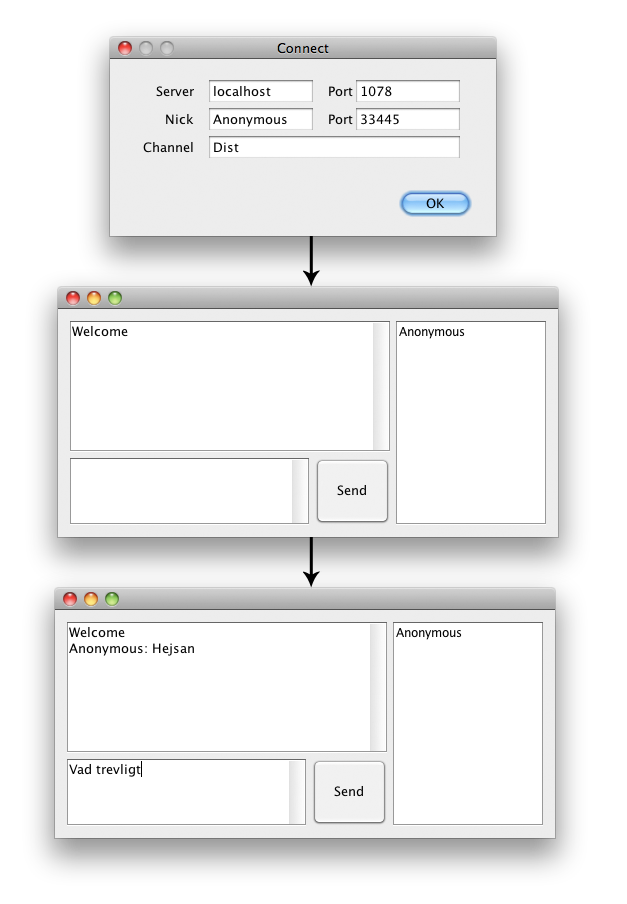
\includegraphics[width=3.3in]{images/TestProgram.png}
  \caption{GUI-application example }
  \label{fig:images/guiapp}
\end{figure}



\section{System description}\label{sec:system}
% Beskriv översiktligt hur programmet är uppbyggt och hur det löser
% problemet.

% The GCom middleware consists of three (logical) modules, the group
% management module, the communication module and the message ordering
% module. These are, respectively, responsible for handling group
% membership issues, communication message exchange semantics and
% message (re)ordering issues. All of these modules need to function
% properly in order for your system to be able to ensure correct
% message delivery semantics.

The \textit{GCom} middlewares distributed network consist of one
\textit{Group Name System} (GNS), \textit{group views} and
\textit{group members}. Each \textit{group views} contains
one or more \textit{group members} and one of these
\textit{group members} servers as \textit{group leader}.
The \textit{GNS} has no other knowledge of the \textit{group views}
except for a referens to the \textit{group leader}.

\subsection{Remote Method Invocation}\label{sec:rmi}
To keep track of the groups, the \textit{GNS} has a referens to a
remote object that represent each groups leader.

Each group member has a referens to a remote object representing the
GNS and one for each other group member. This means all group members
are connected to each other.

\begin{figure}[!thb]
  \centering
  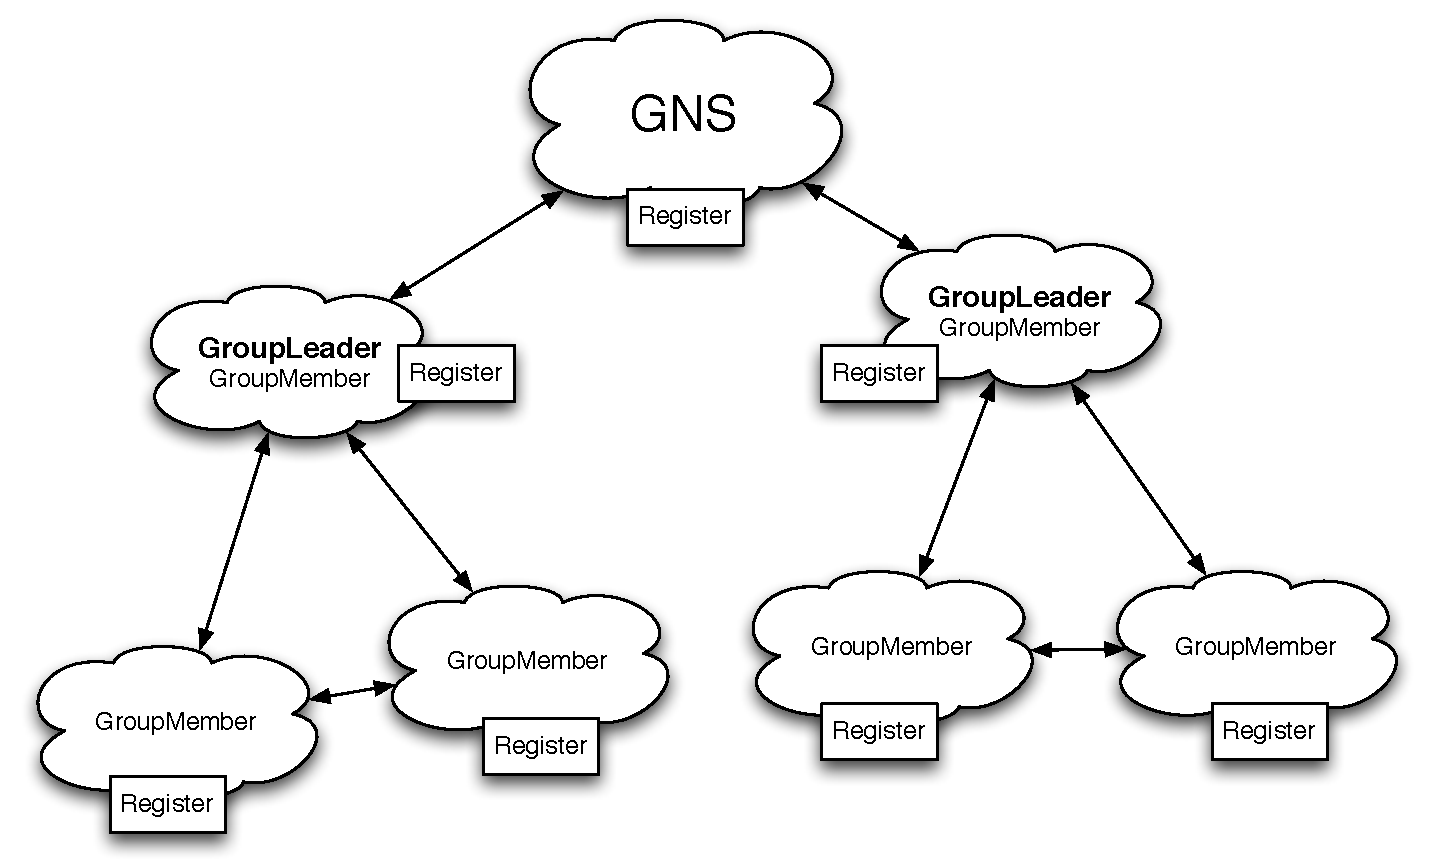
\includegraphics[width=3.3in]{images/Overview.pdf}
  \caption{GCOM overview}
  \label{fig:images/overview}
\end{figure}


\subsection{The modules}\label{sec:modules}

The \textit{GCom} middleware is separated in three different modules
to separate different behaviours, see figure \vref{fig:images/Stack}.
The first module which will have the closest connection to
implementing software is the \textit{management module}. This module
handles group membership changes and actions. The second module
\textit{ordering module}, handles message ordering. The third module
\textit{communications module} is the one that actually sends and
receives messages to and from the group. These modules will be
discussed in more detail in the following sections.

% \begin{figure}[!t]
%   \centering
%   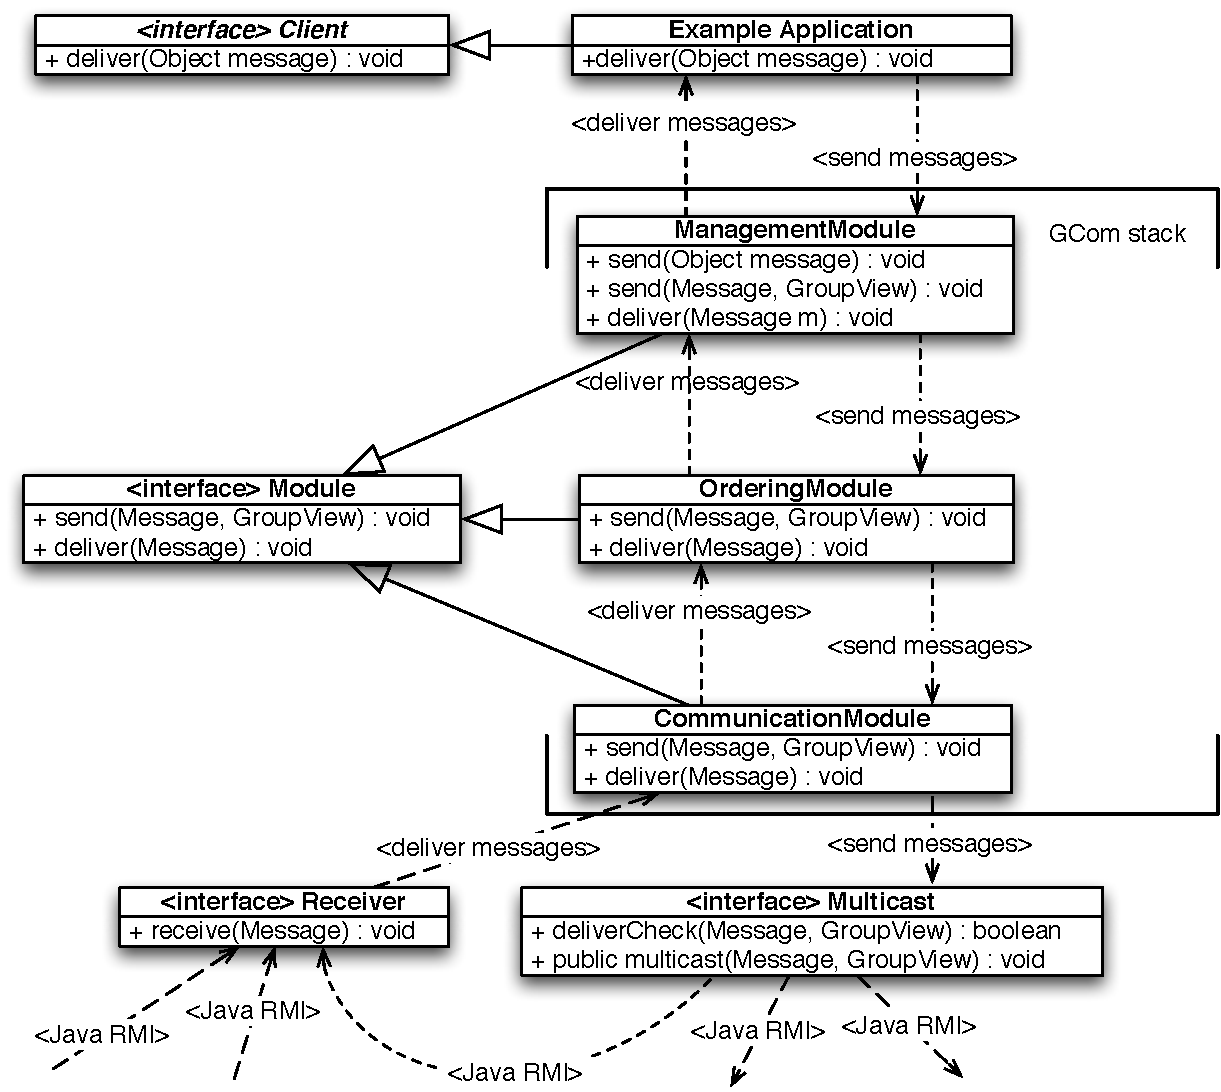
\includegraphics[width=2.5in]{images/Stack.pdf}
%    %   \centerline{\subfloat[Case I]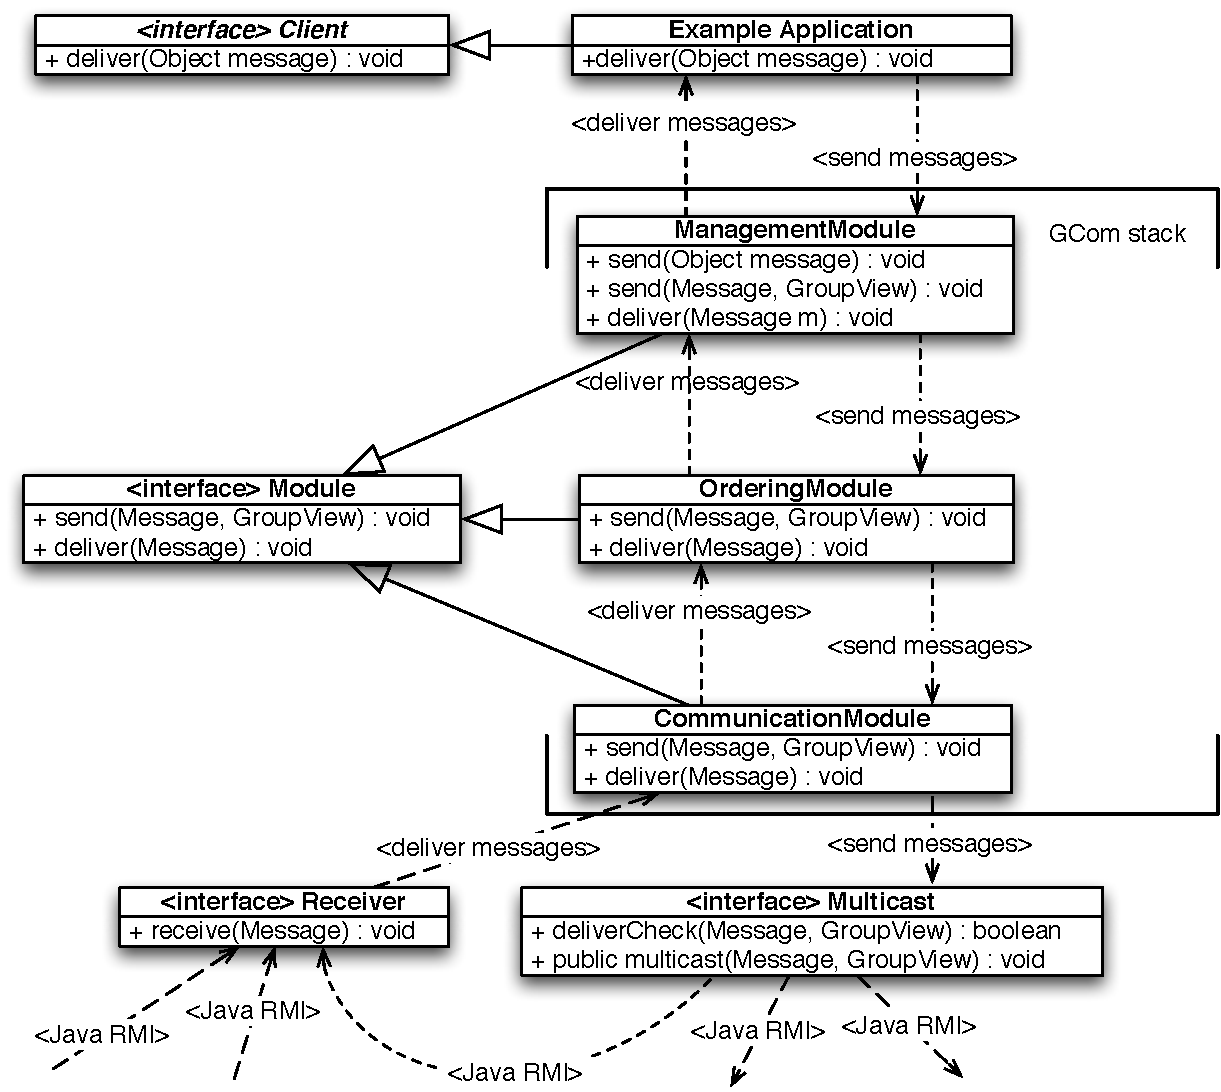
\includegraphics[width=2.5in]{images/Stack.pdf}}
%   \caption{GCom stack}
%   \label{fig:images/Stack}
% \end{figure}

\begin{figure*}[!thb]
  \centerline{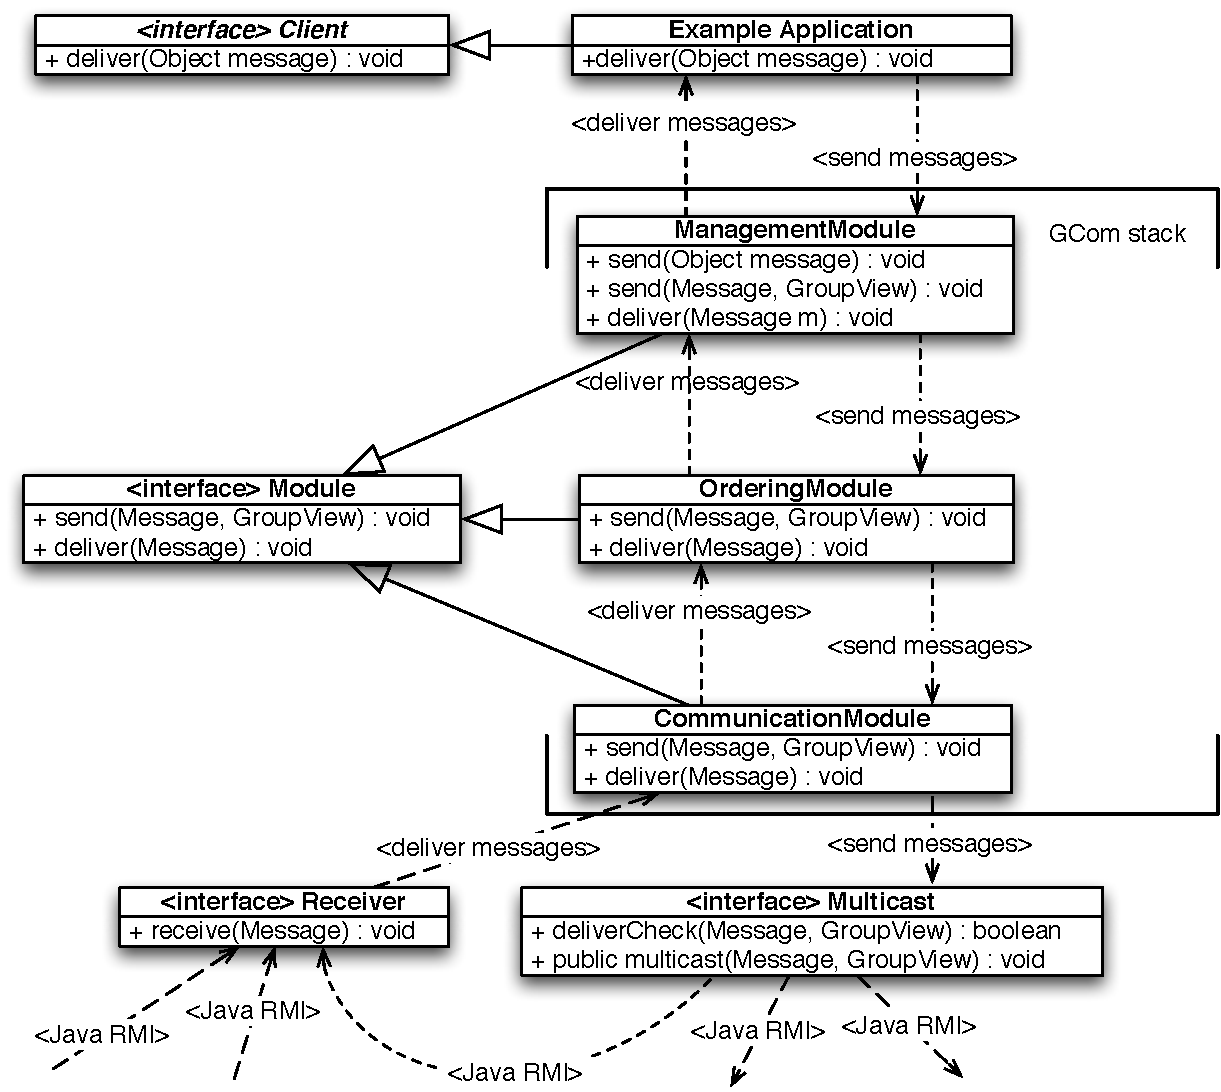
\includegraphics[width=110mm]{images/Stack.pdf}}
  \caption{GCom stack}
  \label{fig:images/Stack}
\end{figure*}

\subsection{Group Name System}\label{sec:group-name-system}
% To resolve group names: When a process sends a message to the group,
% the group management module resolves the group name into a list of
% group members.
To act as an entry point for group members in a \textit{GCom} system
there must be an instance of \textit{se.umu.cs.jsgajn.gcom.GNS}
running on a machine with a known address. The \textit{GNS} acts as a
Group Name System service which means that it resolves a group name
consisting of string, to an instance of the remote interface of the
group leader.

When a process wants to connect it provides a groupname and if
the group exists, the \textit{GNS} returns the instance of the group
leaders remote interface. If the group doesn't exist a new group is
created and the connecting process is assigned as group leader.

The \textit{GNS} is \textit{GCom} only critical point of failure. If
the \textit{GNS} crashes no new group members can join groups without
an instance of any group members remote interface.

If the \textit{GNS} where to crash it can be started once again with
a serialized object of the groups it contained before the crash. This
is done with the following command:\\
\begin{footnotesize}
  \verb!salt:./GCom> java -jar GCom.jar GroupSettingMap.ser!
\end{footnotesize}\\
The previous command provides the \textit{GNS} with a file
\textit{GroupSettingMap.ser} which is saved by the last instance of a
running \textit{GNS}.

\subsection{Group management module}\label{sec:group-management-module}
The \textit{group management module} is the top one in the application
stack, see figure \ref{fig:images/Stack}. Software using the
\textit{GCom} middleware will should handle all communication through
this module by creating an instance of it and passing an instance of
\textit{se.umu.cs.jsgajn.gcom.Client} to the constructor of the
\textit{Group management module}.

A newly created \textit{group management module} will initialize all
other modules needed for a fully functional \textit{GCom} application
stack.

The default implementation of the \textit{group management module} is
implemented in the class (package truncated):\\
\textit{s.u.c.j.g.management.ManagementModuleImpl}.\\
This implementation will contain one thread to send messages and one
thread to receive messages. All messages to be sent are first paced in
a priority queue where all messages are ordered according to the
\textit{first in first out} principle, except some system messages
that are prioritized before client messages. The system are those sent
when a process wants to join a group, the message sent when a group
constellation has changed and when a member has detected that another
member has crashed.

\subsubsection{Group leaders}\label{sec:group-leaders}
% To provide an interface for group management: The group management
% module provides operations to create and remove groups, as well as
% add and remove members from a group.
Since groups may contain large amounts of group members the
\textit{GNS} only contains a reference to one of the group members.
This member is called the group leader. A group leader is responsible
for receiving and managing joining members. In the case of the total
ordering of messages the group leader will act as a sequencer for the
group, see section \ref{sec:total}.

\subsubsection{Error handling}\label{sec:error-handling}
% To detect errors: The module monitors a group and indicates when a
% member of the group crashes (or for some other reason become
% unreachable).
When sending messages a group member may detect that one of the
receiving members has crashed. If the detecting member is a group
leader it will directly send a groupchange message, otherwise it will
send a membercrash message which when received by the group leader
will result in a groupchange message multicasted to the group. A
groupchange message contains information about the complete new group
composition whereas a membercrash message only contains information
about the members that have crashed.

When the member that has crashed is the group leader the exact same procedure is used except that when processes receive membercrash messages they will check if they are the new group leader, and if they are they will send a groupchange message to the group. Group members test if they are the new group leader by checking if they have the maximum value of \textit{UUID}s in the current group. This is a variant of the \textit{Bully alghoritm}, see page 482 \cite{book:dist-syst}.

% TODO: this section maybe should have contained info about normal leave
% messages, which we have not implemented.
% \subsubsection{Group changes}\label{sec:group-changes}
% To notify changes in group membership: The module notifies all group
% members about changes in group composition.

\subsection{Message ordering module}\label{sec:message-ordering-module}
The \textit{Message ordering module} is responsible for message
ordering. That is it will for different orderings guarante that all
messages delivered from this module up to the group \textit{management
  module} is order according to the current ordering. The
\textit{management module} will send all outgoing messages to this
module, which will prepare the message with necessary information such
as vector-clocks and pass the message along to the
\textit{communications module}. The \textit{communications module}
will in turn deliver received messages from other group members
through the \textit{ordering module}. When messages are delivered here
they are immediately put in the current ordering implementation. All
ordering implementations describe in the following sections act as
\textit{BlockingQueue}\footnote{\url{http://java.sun.com/j2se/1.5.0/docs/api/java/util/concurrent/BlockingQueue.html}}.
When taking messages from them they block until they can release a
message which confirms to their message ordering guarantee.

\begin{figure}[!thb]
  \centering
  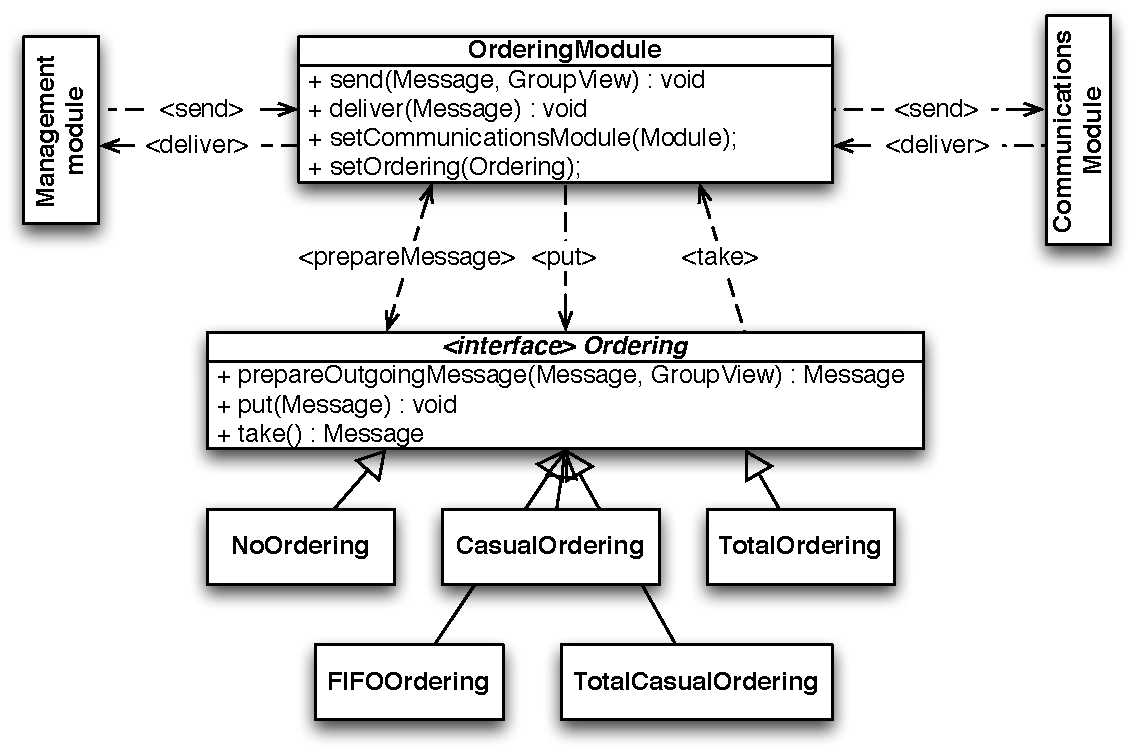
\includegraphics[width=3.3in]{images/Ordering.pdf}
  \caption{Ordering module}
  \label{fig:images/ordering}
\end{figure}

Because \textit{GCom} is implemented to allow members to join already
existing groups the different type of orderings handle their first
ever message from a group member as a starting point for ordering
subsequent messages. This means that if a message is received after
the first message that should have been received before the first
message, it is discarded.

\subsubsection{Non-ordered}\label{sec:-non-ordered}
The \textit{non-ordered} ordering does not make any guarantee about
the ordering of messages. It do however release messages it receives
in the exact same order as it gets them.

\subsubsection{FIFO ordering}\label{sec:fifo}
The \textit{FIFO} ordering will release messages received from a
correct process in the same order as they are sent from that process.
This is done by keeping a counter of how many messages it has
delivered for each group member. When preparing an outgoing message
\textit{FIFO} will piggyback onto that message the total number of
messages it has prepared and sent. When receiving a message
\textit{FIFO} compares the counter in the message with its own receive
counter for the sending message. If the message is not the next in
order for that sender, the message will be put in a hold-back queue
until it is.

Table \ref{tbl:fifo} shows a scenario where one process \textit{p3}
receives all messages in the reverse order they are sent, this results
in an \textit{FIFO} order for message from the same sender but
messages from different senders are not guaranteed to be delivered in
the same order for all processes.

\begin{table}[H]
  \centering
  \begin{footnotesize}
    \begin{tabular} {c | c | c | c}
      % BEGIN RECEIVE ORGTBL fifo
      & p1 & p2 & p3 (hold all messages) \\
      \hline
      Send order & one &  &  \\
      &  & 2 &  \\
      & three &  &  \\
      &  & 4 &  \\
      \hline
      &  &  & (Release messages in reverse order) \\
      \hline
      Receive order & one & one & 2 \\
      & 2 & 2 & 4 \\
      & three & three & one \\
      & 4 & 4 & three \\
      % END RECEIVE ORGTBL fifo
   \end{tabular}
  \end{footnotesize}
  \caption{Fifo ordering tests}
  \label{tbl:fifo}
\end{table}
\begin{comment}
  #+ORGTBL: SEND fifo orgtbl-to-latex :splice t
  |               | p1    |    p2 | p3 (hold all messages)              |
  |---------------+-------+-------+-------------------------------------|
  | Send order    | one   |       |                                     |
  |               |       |     2 |                                     |
  |               | three |       |                                     |
  |               |       |     4 |                                     |
  |---------------+-------+-------+-------------------------------------|
  |               |       |       | (Release messages in reverse order) |
  |---------------+-------+-------+-------------------------------------|
  | Receive order | one   |   one | 2                                   |
  |               | 2     |     2 | 4                                   |
  |               | three | three | one                                 |
  |               | 4     |     4 | three                               |
\end{comment}


\subsubsection{Causal ordering}\label{sec:causal}
The \textit{Casual} ordering guarantees that messages will be ordered
by a cause and event ordering. That is if one message is sent as a
reply to another message all members will deliver those messages in
the correct order. More formally from \cite{book:dist-syst}:
\textit{''If multicast(g, m) $\rightarrow$ multicast(g, m'), where
  $\rightarrow$ is the happened-before relation induced only by
  messages sent between the members of g, then any correct process
  that delivers m' will deliver m before m' ''}.

This is done by letting each group member keep track of the number of
messages it has delivered from each other group member as well as
keeping a counter for the number of messages it has sent to the group.
This record of message counters is called a \textit{vector-clock}, see
page 447 \cite{book:dist-syst}.

When preparing a message for sending every process piggybacks its
vector clock on the outgoing message.

When receiving a message \textit{Casual} ordering places the message
in a hold back queue until it the next to be delivered from the
sending member, and it has delivered all messages that the sending
member had delivered when sending that message.

Table \ref{tbl:casual} shows a scenario where process \textit{p3} receives all messages in the reverese order from which they are sent. This results in a \textit{casual} order where all messages are ordered according to the messages delivered by the sending processes at send time. All messages are in order for process \textit{p3} except message \textit{V} since no process had delivered that message when sending the other messages.

\begin{table}[H]
  \centering
  \begin{footnotesize}
    \begin{tabular} {c | c | c | c}
      % BEGIN RECEIVE ORGTBL casual
      & p1 & p2 & p3 (hold all messages) \\
      \hline
      Send order & one &  &  \\
      &  & 2 &  \\
      & three &  &  \\
      &  & 4 &  \\
      &  &  & V \\
      \hline
      &  &  & (Release messages in reverse order) \\
      \hline
      Receive order & one & one & V \\
      & 2 & 2 & one \\
      & three & three & 2 \\
      & 4 & 4 & three \\
      & V & V & 4 \\
      % END RECEIVE ORGTBL casual
    \end{tabular}
  \end{footnotesize}
  \caption{Casual ordering tests}
  \label{tbl:casual}
\end{table}
\begin{comment}
  #+ORGTBL: SEND casual orgtbl-to-latex :splice t
  |               | p1    |    p2 | p3 (hold all messages)              |
  |---------------+-------+-------+-------------------------------------|
  | Send order    | one   |       |                                     |
  |               |       |     2 |                                     |
  |               | three |       |                                     |
  |               |       |     4 |                                     |
  |               |       |       | V                                   |
  |---------------+-------+-------+-------------------------------------|
  |               |       |       | (Release messages in reverse order) |
  |---------------+-------+-------+-------------------------------------|
  | Receive order | one   |   one | V                                   |
  |               | 2     |     2 | one                                 |
  |               | three | three | 2                                   |
  |               | 4     |     4 | three                               |
  |               | V     |     V | 4                                   |
\end{comment}

\subsubsection{Total ordering}\label{sec:total}
Total order makes all the processes in the system to deliver all messages
in the same order. This doesn't mean it's the right order, but it is the same.
This is possible by letting the group leader become a sequencer. This means
that all messages in the system have to ask the leader for a sequence number
before they can multicast their messages. Then all processes have to order
incoming messages after this sequence numbers.

Table \ref{tbl:total} show a scenario where process \textit{p3}
receives all messages in the reverse order from which they are sent.
This does not effect the outcome at all, messages are delivered at all
processes in the same order.

Table \ref{tbl:totalseq} show a scenario where the sequencer deliveres
sequence numbers in the reverese order for which they are received.
This results in a reverse order for all processes.
\begin{table}[H]
  \centering
  \begin{footnotesize}
    \begin{tabular} {c | c | c | c}
      % BEGIN RECEIVE ORGTBL total
      & p1 & p2 & p3 (hold all messages) \\
      \hline
      Send order & one &  &  \\
      &  & 2 &  \\
      & three &  &  \\
      &  & 4 &  \\
      &  &  & V \\
      \hline
      &  &  & (Release messages in reverse order) \\
      \hline
      Receive order & one & one & one \\
      & 2 & 2 & 2 \\
      & three & three & three \\
      & 4 & 4 & 4 \\
      & V & V & V \\
      % END RECEIVE ORGTBL total
    \end{tabular}
  \end{footnotesize}
  \caption{Total ordering tests}
  \label{tbl:total}
\end{table}
\begin{comment}
  #+ORGTBL: SEND total orgtbl-to-latex :splice t
  |               | p1    |    p2 | p3 (hold all messages)              |
  |---------------+-------+-------+-------------------------------------|
  | Send order    | one   |       |                                     |
  |               |       |     2 |                                     |
  |               | three |       |                                     |
  |               |       |     4 |                                     |
  |               |       |       | V                                   |
  |---------------+-------+-------+-------------------------------------|
  |               |       |       | (Release messages in reverse order) |
  |---------------+-------+-------+-------------------------------------|
  | Receive order | one   |   one | one                                 |
  |               | 2     |     2 | 2                                   |
  |               | three | three | three                               |
  |               | 4     |     4 | 4                                   |
  |               | V     |     V | V                                   |
\end{comment}

\begin{table}[H]
  \centering
  \begin{footnotesize}
    \begin{tabular} {c | c | c | c}
      % BEGIN RECEIVE ORGTBL totalB
      & p1 & p2 & p3 - Sequencer (hold all messages) \\
      \hline
      Send order & one &  &  \\
      & two &  &  \\
      \hline
      &  &  & (Release messages in reverse order) \\
      \hline
      Receive order & two & two & two \\
      & one & one & one \\
      % END RECEIVE ORGTBL totalB
    \end{tabular}
  \end{footnotesize}
  \caption{Total ordering tests}
  \label{tbl:totalseq}
\end{table}
\begin{comment}
  #+ORGTBL: SEND totalB orgtbl-to-latex :splice t
  |               | p1  | p2  | p3 - Sequencer (hold all messages)  |
  |---------------+-----+-----+-------------------------------------|
  | Send order    | one |     |                                     |
  |               | two |     |                                     |
  |---------------+-----+-----+-------------------------------------|
  |               |     |     | (Release messages in reverse order) |
  |---------------+-----+-----+-------------------------------------|
  | Receive order | two | two | two                                 |
  |               | one | one | one                                 |
\end{comment}

\subsubsection{Causal-Total ordering}\label{sec:causal-total}
% (messages are first sorted according to causal ordering, then
% according to total ordering)
The \textit{Casual-total} ordering is almost identical to
\textit{Total} ordering except that the sequencer will use an instance
of the \textit{FIFO} ordering implementation to make sure that before
sending out sequences number for requests, the requests should first
be casualy ordered. This means that all messages delivered in the
group are both casualy and totaly ordered. For a discussion about the
reasoning behind using a \textit{FIFO} instead of a \textit{Casual}
ordering in the sequencer, see section \ref{sec:disc-casual-total}.

Table \ref{tbl:castot} shows a scenario where the sequencer receives messages in reverse order. This does not affect the sequence numberse released from the sequencer since they are first \textit{FIFO} ordered.

\begin{table}[H]
  \centering
  \begin{footnotesize}
    \begin{tabular} {c | c | c | c}
      % BEGIN RECEIVE ORGTBL casualtotal
      & p1 & p2 & p3 - Sequencer (hold all messages) \\
      \hline
      Send order & one &  &  \\
      & two &  &  \\
      \hline
      &  &  & (Release messages in reverse order) \\
      \hline
      Receive order & one & one & one \\
      & two & two & two \\
      % END RECEIVE ORGTBL casualtotal
    \end{tabular}
  \end{footnotesize}
  \caption{Casual-Total ordering tests}
  \label{tbl:castot}
\end{table}
\begin{comment}
  #+ORGTBL: SEND casualtotal orgtbl-to-latex :splice t
  |               | p1  | p2  | p3 - Sequencer (hold all messages)  |
  |---------------+-----+-----+-------------------------------------|
  | Send order    | one |     |                                     |
  |               | two |     |                                     |
  |---------------+-----+-----+-------------------------------------|
  |               |     |     | (Release messages in reverse order) |
  |---------------+-----+-----+-------------------------------------|
  | Receive order | one | one | one                                 |
  |               | two | two | two                                 |
\end{comment}


\subsection{Communications module}\label{sec:communications-module}
The \textit{communications module} is responsible for the actual
sending and receiving of messages for a group member. All
communication is done through \textit{Java RMI} by calling methods on
remote objects.

A \textit{communications module} will use an instance of a
\textit{Multicast} interface to multicast messages to a group. Two
multicast methods are implemented, \textit{Basic multicast} and
\textit{Reliable multicast}, see figure \ref{fig:images/commodule}.

\begin{figure}[!thb]
  \centering
  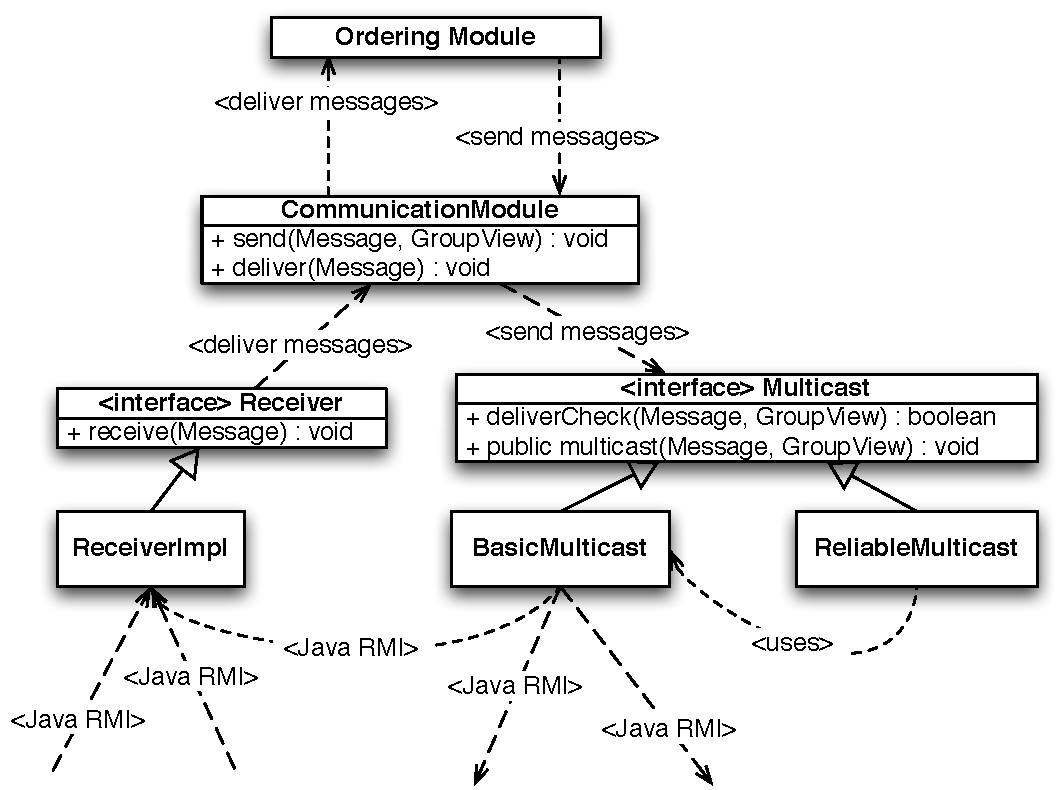
\includegraphics[width=3.3in]{images/ComModule.pdf}
  \caption{Communications module}
  \label{fig:images/commodule}
\end{figure}

\subsubsection{Basic multicast}\label{sec:basic-multicast}
The multicast method \textit{Basic multicast} makes no guarantee that
all members of a group will receive a message sent. Sending messages
is done with \textit{one-to-one} communication with every member of
the group. If for example the process where to fail when halfway
through sending messages to the group, then the reminding half of the
group will never receive that message. This is handled by
\textit{Reliable multicast}.

\subsubsection{Reliable multicast}\label{sec:reliable-multicast}
The multicast method \textit{Reliable multicast} guarantee that a
message delivered at one correct process is delivered at all correct
processes.

\subsection{Debugger}\label{sec:debugger}
% That messages are delivered according to the specified ordering

% How messages are propagated in the network: Show both the path a
% message takes and how many times a certain process has received a
% certain message.

% The content of hold-back queues and other buffers: Present all
% messages waiting to be sent or delivered as well as values of vector
% clocks and other counters.

% Current system performance: As a measure of the system performance,
% count the number of messages (including control messages) required
% to perform an operation (send one message with certain ordering and
% certain multicast).

The debugger is a singelton and works as an entirely independent
application. It can be activated in all classes of GCOM and it has a
lot of useful functions. The debugger is uniq for the group member
that starts it, that means it montors only the things which that group
member.

The debugger can be used to reproduce the ordering examples in the
tables \ref{tbl:fifo}-\ref{tbl:castot}. The interface is shown in
figure \vref{fig:images/Debuggerstart} and figure
\vref{fig:images/holdqueues}.

\subsubsection{Debugger functions}\label{sec:debuggerfunctions}
Here is a list of all the functions in the debugger.
\begin{itemize}
\item Table with all received messages including this info
  \begin{itemize}
  \item Number of times the message been received
  \item Short id (all message receives a debugger-id 1,2,3++)
  \item UUID
  \item Message content
  \item Original sender UUID
  \item The message-object
  \item Doubleclick : Path message has taken, is it a
    systemmessage, its sequencenumber
  \end{itemize}
\item List all delivered messages including this info
  \begin{itemize}
  \item Short id (all message receives a debugger-id 1,2,3++)
  \item UUID
  \item Message content
  \item Original sender UUID
  \item The message-object
  \item Doubleclick : Path message has taken, is it a
    systemmessage, its sequencenumber
  \end{itemize}
\item Information internal vector clock
\item List of the members in the current group view
\item Hold/unhold  messages from being delivered to the client
\item Shuffle or revers the hold queue
\item Release one or all messages from the holdqueue
\item Table with all de helded messages
  \begin{itemize}
  \item Message content
  \item UUID
  \end{itemize}
\item Table with the messages that is currently held in the
  ordering-class (except for the CasualTotal-ordering)
  \begin{itemize}
  \item Message content
  \item UUID
  \end{itemize}
\item Possibility to let two messages when using the
  CasualTotal-ordering change order before goring to the sequencer.
\end{itemize}

\begin{figure*}[!thb]
  \centerline{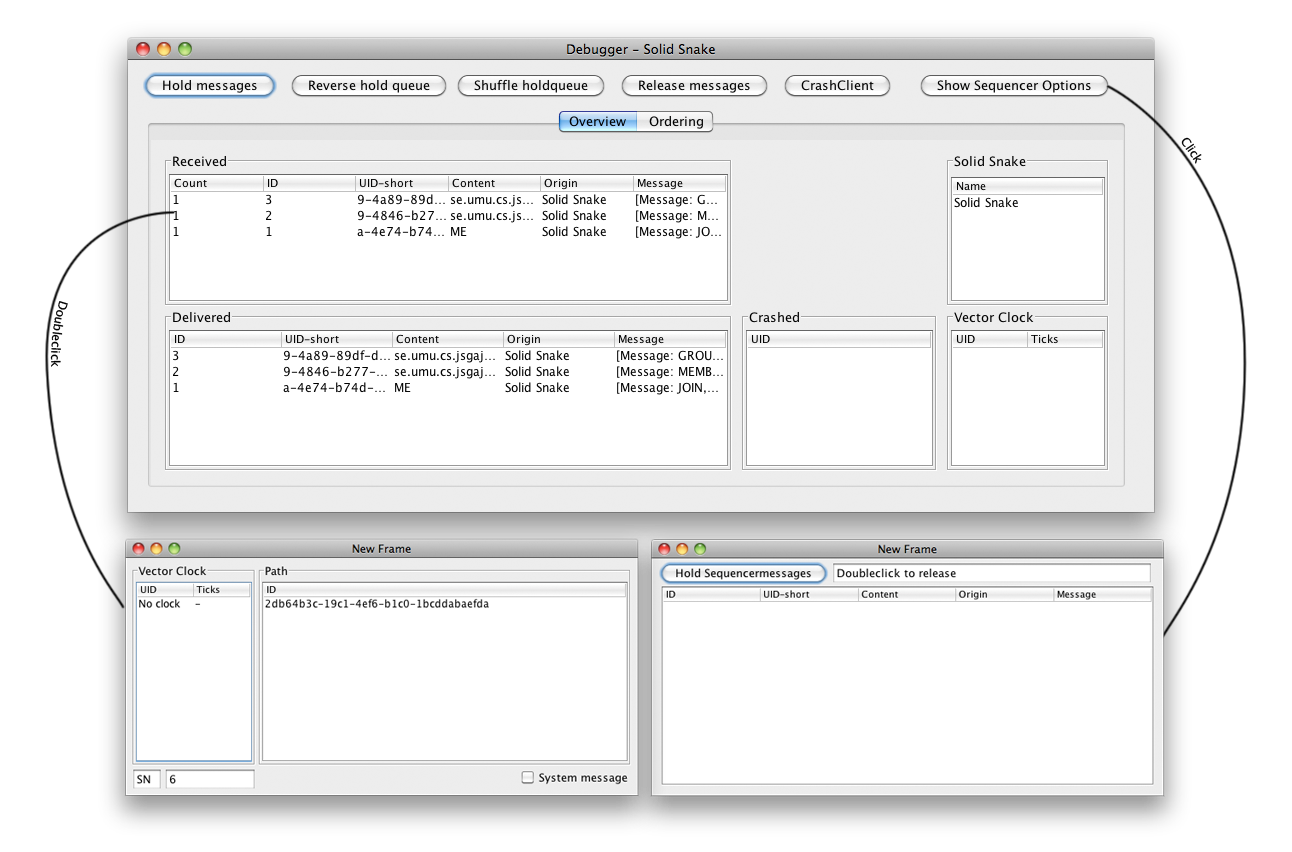
\includegraphics[width=150mm]{images/Debuggerstart.png}}
  \caption{Debugger start screen with popups}
  \label{fig:images/Debuggerstart}
\end{figure*}

\begin{figure}[!thb]
  \centering
  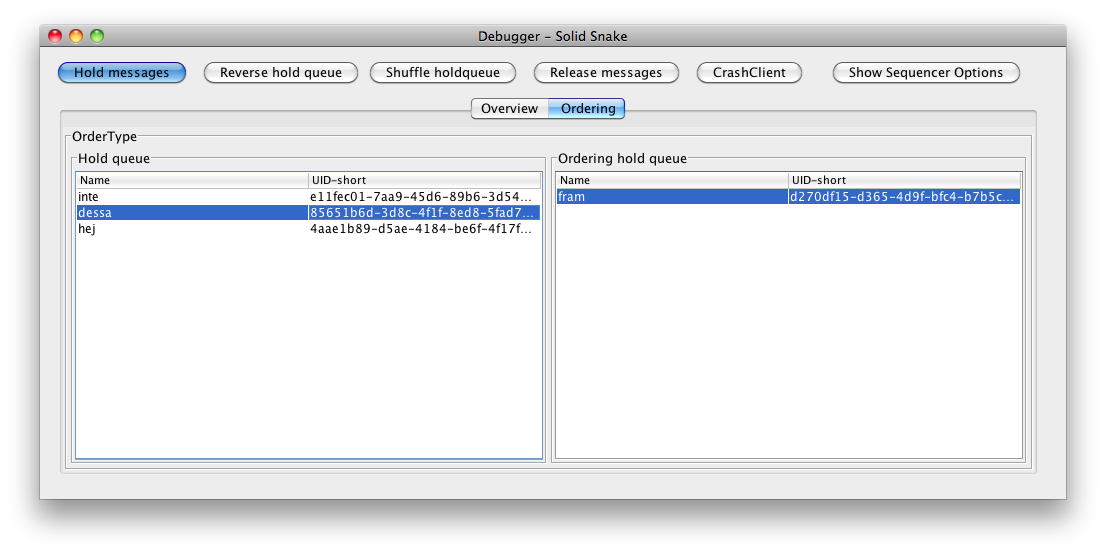
\includegraphics[width=3.3in]{images/Holdqueues.png}
  \caption{Debugger hold queues}
  \label{fig:images/holdqueues}
\end{figure}


\section{Discussion}\label{sec:discussion}
% Vilka problem och begränsningar har din lösning av uppgiften? Hur
% skulle de kunna rättas till?
The following sections will discuss some of the problems and solutions
encountered while implementing \textit{GCom}.

\subsection{Casual-Total ordering}\label{sec:disc-casual-total}
The \textit{Total} ordering in our implementation of \textit{GCom}
doesn't allow group members to multicast messages without first having
piggybacked a correct sequence number to the message. This implies
that because our first implementation only had one sending thread
there would not exist any case where a message got an a sequence
number which was not both total and casual.

To make a different between the total order and the total-casual
ordering as defined by the assignment specification we made it
possible for the process to use multiple processes to simultaneously
send messages. This way there can exist a case where a message on its
way to the sequencer will be surpassed by a later message from the
same process. That would in a totaly orderd system mean that the
messages would be received in the reverse order, but our total-casual
sequencer will FIFO order the messages back to their original order
before giving them sequence numbers.

\subsection{Passing remote objects}\label{sec:passing-remote-ojbects}
Our implementation pass remote objects directly between different
processes to enable group members to get a connection to other group
members. This could become a problem on systems that are connected to
internet behind a firewall. Since the lookup of the remote object only
is done once different hosts might not have an open route to a process
behind a firewall.
% \section{Reflektioner}\label{Reflektioner}
% % Reflektioner - Var det något som var speciellt krångligt? Vilka
% % problem uppstod och hur löste ni dem? Vilka verktyg använde ni? Hur
% % upplevde ni de verktygen? + Allmänna synpunkter. Om ni har upplevt
% % problem på grund av olika miljöer (i termer av operativsystem och
% % liknande) så kan det även vara intressant att nämna det, samt motivera
% % ert val av miljö.

\subsection{No automatic failure detection}\label{sec:no-automatic-failure-detection}
We have no automatic "ping-function" in our system. That means that if for example
a group member crashed, no one will realize this before they tries to send a message. This also
implies that if the leader crashes and no messages is sent, there will be no way to connect to the group.

\subsection{Security}\label{sec:security}
Here there are great opportunities for development. For instance, teoreticly anyone could send I 
GroupChange-message and noone will know it the sender is the leader or not. It is the same way 
with all other messages types.

\section{Scenarios}\label{sec:scenarios}
This section shows different scenarios that explains how the system
works.

\subsection{Create new group}
P = The process that wants to create new group.
\begin{enumerate}
\item P: Create GroupSettings-object with information about name,
  leader (the process itself) orderingtype and multicasttype.
\item P: Create a remote object of the GNS.
\item P: Connect to the GNS with the GroupSettings-object.
\item GNS: Saves the GroupSetting-object and then returns it to the
  process again (with a notice if its new or if the group already
  existed, in this scenario we presume the group didn’t existed).
\item P: Creates a GroupLeaderImpl()-instance.
\item P: Starts the receive- and senderthreads.
\end{enumerate}

\subsection{Join existing group}
P = The process that wants to join new group. GL = GroupLeader
\begin{enumerate}
\item P: Create GroupSettings-object with information about name,
  leader (the process itself) orderingtype and multicasttype.
\item P: Create a remote object of the GNS.
\item P: Connect to the GNS with the GroupSettings-object.
\item GNS: Discovers that I group with the given name already exist
  and then returns the already saved group.
\item P: Create a join-message and inserting a remote object referring
  to itself as message content.
\item P: Creates new GroupView with the leader from the
  GroupSettings-object.
\item P: Sends the join-message to the OrderingModule where it skips
  the ordering because it counts as an system message.
\item P: CommunicationModel receives the message from ordering module
  and then multicasts it.
\item All members: Receives the message.
\item GL: Adds new member to current GroupView-object.
\item GL: Create a GroupChange with the updated GroupView-object as content.
\item GL: Multicasts the message to all members (this message is also
  a system messages which makes it skip ordering)
\item All members: Receives GroupChange-message and updates thier groups
\end{enumerate}

\subsection{Member crash (not leader)}
P = The process that discovers crashed member. GL = GroupLeader
\begin{enumerate}
\item P: Tries to multicast message to process C and discovers I
  remote exception because C has crashed.
\item P: Throws MemberCrashException which includes C.
\item P: ManagementModule catches the Exception.
\item P: Creates MemberCrash-messages with C as its content and
  multicasts it to the group view (this is I system message which
  means it skips ordering)
\item All members: Receives message.
\item GL: Removes C from it’s GroupView.
\item GL: Create a GroupChange with the updated GroupView-object as content.
\item GL: Multicasts the message to all members (this message is also
  a system messages which makes it skip ordering)
\item All members: Receives GroupChange-message and updates their groups.
\end{enumerate}
Note: Some other member in the group will maybe also discovers that C
has crashed so this reaction chain may be executed more times than
one.

\subsection{Leader crash}
P = The process that discovers the crashed leader. GL = GroupLeader
\begin{enumerate}
\item P: Tries to multicast message to process C and discovers I
  remote exception because C has crashed.
\item P: Throws MemberCrashException which includes C.
\item P: ManagementModule catches the Exception.
\item P: Creates MemberCrash-messages with C as its content and
  multicasts it to the group view (this is I system message which
  means it skips ordering)
\item All members: Receives message.
\item All members: Discovers that is the leader that is dead, then
  removes the leader from their group view.
\item All members: Checks if their own MangagementModule has the
  highest UUID in the GroupView.
\item Member with highest UUID: Notifys the GNS that the group has a new leader.
\item GNS: Updates it’s leaderreferens for the group
\item GL (new): Creates a GroupLeaderImpl-instance.
\item GL: Create a GroupChange with the updated GroupView-object as content.
\item GL: Multicasts the message to all members (this message is also
  a system messages which makes it skip ordering)
\item All members: Receives GroupChange-message and updates their groups
\end{enumerate}
Note: Some other member in the group will maybe also discovers that C
has crashed so this reaction chain may be executed more times than
one.



\section{Tests}\label{sec:tests}
% Noggranna testkörningar där man ser att programmet fungerar som det
% ska.

% During your demo, you will need to convince the teachers that your
% implementation works. Bring a test protocol, i.e., a series of tests
% that clearly demonstrates that your GCom fulfills the requirements
% and a test tool which can be used to apply it. The test protocol
% should include, e.g., tests of all message orders and multicast
% types. Bring a copy of the test protocol on paper, see page 491 in
% [DS] for suggested notation. Your test protocol must clearly state
% your names, user names, and which level you intend to demonstrate.

% The fact that a system cannot be formally proven to work does not
% make it impossible to implement - consider for example the Internet.
% Read pages 498 and 508 in [DS].



%%%%%%%%%%%%%%%% END APPENDIX AND STUFF %%%%%%%%%%%%%%%%
\bibliographystyle{alpha}
\bibliography{books.bib}

%\newpage
%\appendix
% \pagenumbering{roman}
% \section{Appendix}\label{sec:kallkod}
% % Källkoden ska finnas tillgänglig i er hemkatalog
% % ~/edu/apjava/lab1/. Bifoga även utskriven källkod.

\end{document}
